\likechapter{Вступ}

У даній роботі нами було створено ігри епохи 00х: змійка та тетріс!
Створено це чудо програмної та інженерної думки на базі arduino та світлодіодної матриці 8х8.

Для гри у змійку було виготовлено джойстик \ref{joy} із кнопок, проводів, макетної плати та рук, що нагло претендують на звання "прямі".
По суті, він являв собою кнопки, які при натисканні притягували відповідні виходи до землі (ардуінка була у режимі $INPUT_PULLUP)$.
Нажаль, до того часу, як почалась розробка тетрісу, даний джойстик не дожив :(

\begin{figure}[h]
\center{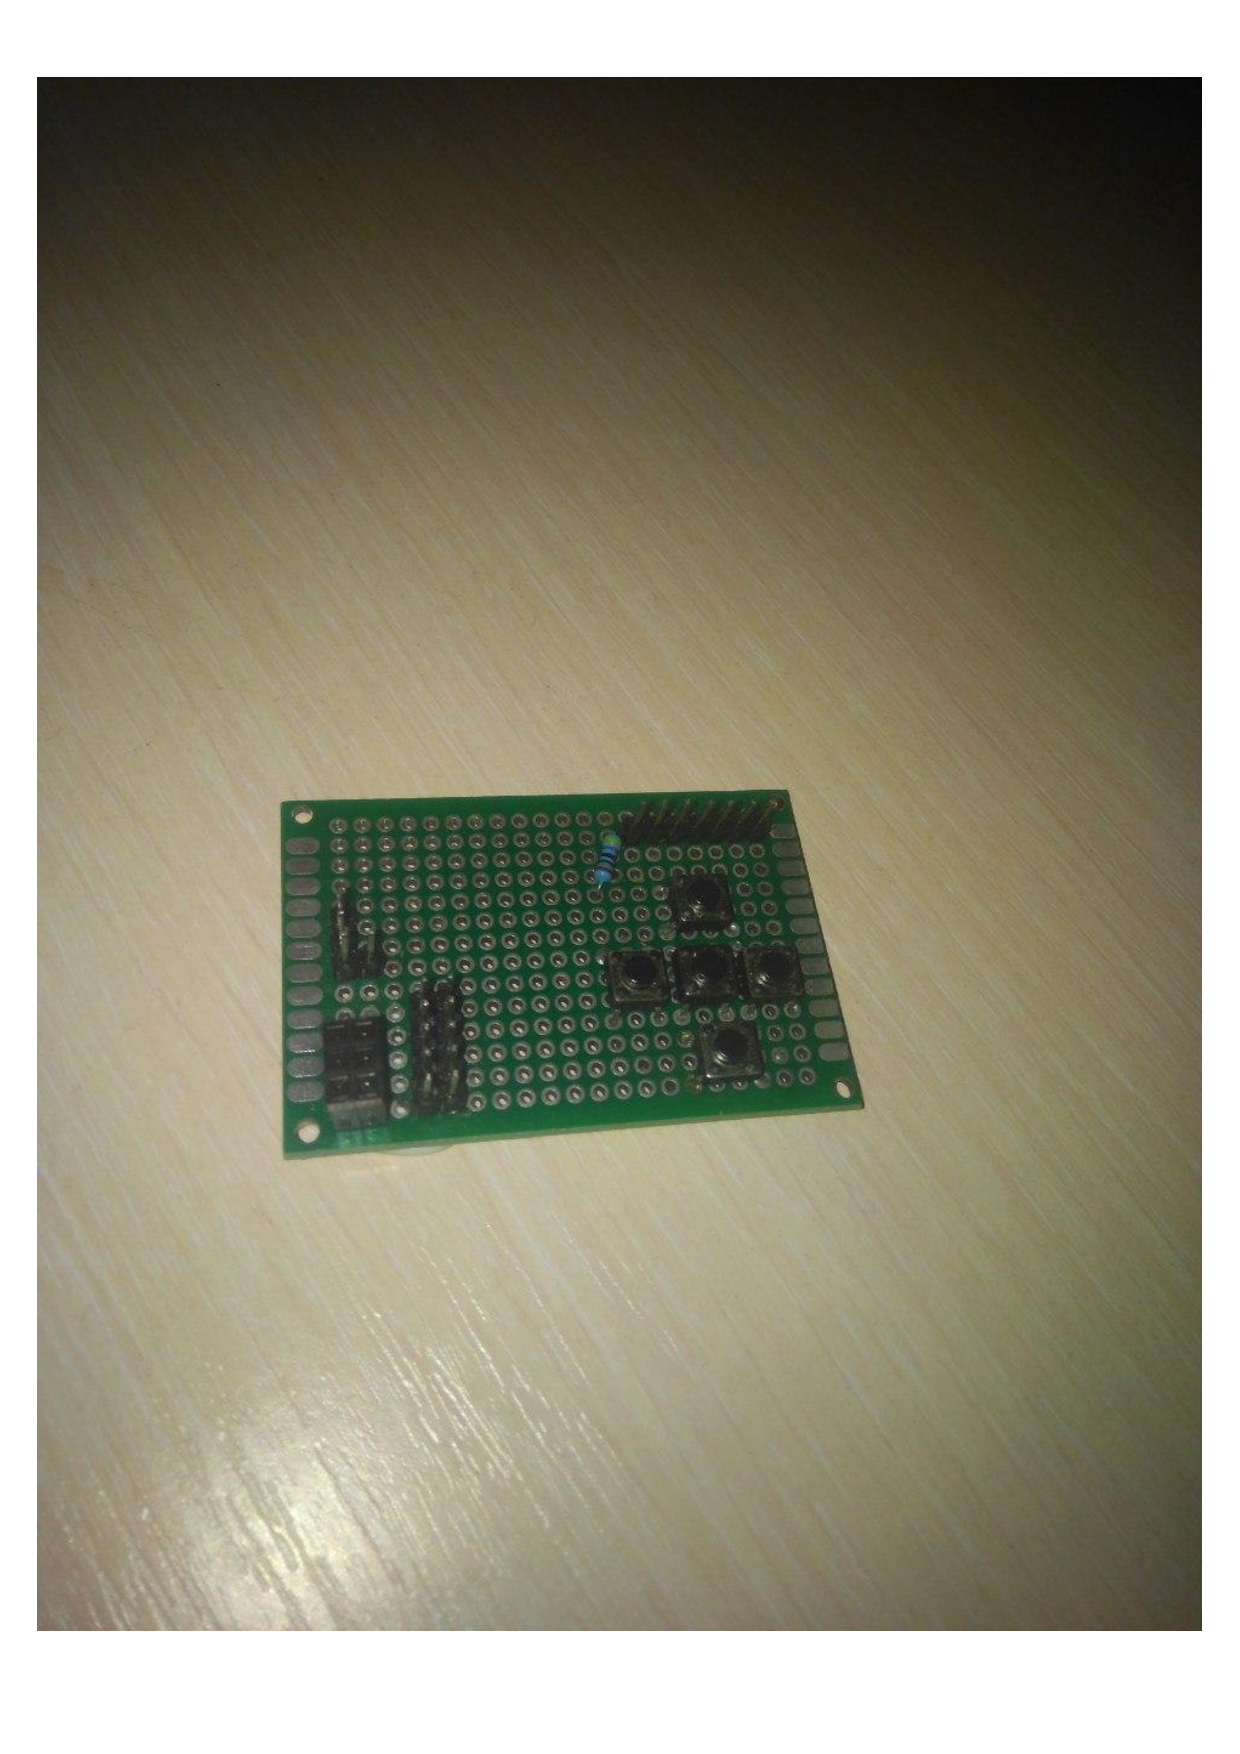
\includegraphics[width=0.9\linewidth]{joy.pdf}}
\caption{Джойстик, що використовувався у змійці.}
\label{joy}
\end{figure}